\documentclass[preprint,12pt]{elsarticle}

\usepackage[utf8]{inputenc}
\usepackage[T1]{fontenc}
\usepackage{amsmath,amssymb}
\usepackage{booktabs}
\usepackage{array}
\usepackage{graphicx}
\usepackage{xcolor}
\usepackage[ruled,vlined,linesnumbered]{algorithm2e}
\usepackage[colorlinks=true,allcolors=blue]{hyperref}
\frenchspacing

% ---- Draft marks: every pending item is red while \draftmarkstrue -------------
\newif\ifdraftmarks
\draftmarkstrue
\definecolor{pending}{HTML}{C00000}
\ifdraftmarks
  \newcommand{\XX}{\textcolor{pending}{\textbf{[XX]}}}
  \newcommand{\pend}[1]{\textcolor{pending}{#1}}
  \newcommand{\placeholder}[1]{\fcolorbox{pending}{white}{\parbox{0.92\linewidth}{\color{pending}\small #1}}}
\else
  \newcommand{\XX}{[XX]}
  \newcommand{\pend}[1]{#1}
  \newcommand{\placeholder}[1]{#1}
\fi

% ---- Notation ----------------------------------------------------------------
\newcommand{\R}{\mathbb{R}}
\newcommand{\vx}{\mathbf{x}}
\newcommand{\vy}{\mathbf{y}}
\newcommand{\vz}{\mathbf{z}}
\newcommand{\vm}{\boldsymbol{\mu}}
\newcommand{\vs}{\boldsymbol{\sigma}}
\newcommand{\vxi}{\boldsymbol{\xi}}
\DeclareMathOperator{\clip}{clip}

\journal{\pend{Venue to be decided}}

\begin{document}

\begin{frontmatter}

% Working title, to be decided with the co-authors.
\title{\pend{Growth laws of a marine bacterium as search rules for continuous
black-box optimization}}

\author{\pend{Authors and affiliations}}

\begin{abstract}
Continuous black-box optimization asks for good solutions when only function
values are available and every evaluation counts against a budget. Many
bio-inspired metaheuristics address it, but their rules usually come from a
qualitative story about the organism and are rarely tested component by
component. We propose the Metaheuristic Algorithm for Regulated Exploration
and Adaptation (MAREA), whose second version, MAREA-2, takes three rules from
laws measured in the marine bacterium \emph{Cobetia} sp.\ MM1IDA2H-1. The fitted logistic growth curve sets the population size schedule, and the
heavy-tailed variability of the growth data sets the shape of the perturbation.
The trade-off between planktonic growth and biofilm formation sets a
success-based step factor and a stagnation-triggered dispersal. We state each rule in
standard optimization terms, next to the mechanism it is equivalent to, and
test it in an ablation study. We compared MAREA-2 with nine algorithms,
including L-SHADE and jSO, on 71 functions from three benchmark suites, in two
dimension settings and at three budgets. MAREA-2 obtained the best mean rank
at the smallest budget in both settings and ranked third, after jSO and
L-SHADE, at the two larger budgets. Against seven classical metaheuristics,
it was significantly better in 40 of 42 signed-rank comparisons. The ablation
attributes the clearest gains to the logistic schedule and the success-based
step factor, and a smaller one to the heavy-tailed perturbation.
\end{abstract}

\begin{keyword}
continuous optimization \sep population size reduction \sep success-based step
adaptation \sep ablation study \sep bacterial growth model \sep benchmarking
\end{keyword}

\end{frontmatter}

% =============================================================================
\section{Introduction}
\label{sec:introduction}

Many design problems in engineering and science reduce to minimizing a function
that can only be evaluated, at some cost, for a given candidate. In continuous
black-box optimization, the algorithm sees neither gradients nor the structure
of the function, and its quality is judged by the solution it finds within a
fixed number of evaluations. Budgets differ by orders of magnitude across
applications. They range from a few thousand evaluations of an expensive
simulator to the $10\,000\,D$ evaluations used in the benchmark competitions of
the IEEE Congress on Evolutionary Computation
(CEC)~\cite{liang2013cec2014,awad2016cec2017,kumar2021cec2022}. An optimizer
that leads at one budget may trail at another, so the budget is part of the
problem statement.

Population-based metaheuristics are the usual tool for this setting. Among the
most reliable are adaptive variants of differential evolution (DE), such as
L-SHADE and jSO~\cite{tanabe2014lshade,brest2017jso}, and the covariance matrix
adaptation evolution strategy (CMA-ES)~\cite{hansen2001cmaes}. Alongside them,
new algorithms inspired by animals, plants, or physical processes appear every
year~\cite{mirjalili2014gwo,heidari2019hho,fu2024sboa}. Their rules are
typically justified by a narrative about the source of inspiration. Several
authors have argued that the narrative often hides known mechanisms, makes the
contribution hard to identify, and replaces a fair comparison with the state of
the art~\cite{sorensen2015metaphor,aranha2022elephant}. A large benchmarking study found that many of these algorithms are
outperformed by random search and that established methods such as CMA-ES, DE,
and L-SHADE remain at the top. The same study found that metaphor-based
algorithms stand out mainly at small budgets~\cite{vermetten2024metaphor}.

The criticism does not imply that a biological source has nothing to offer. It
asks that the source be used on a scientific basis and that the resulting
algorithm be described and tested as an algorithm~\cite{aranha2022elephant}.
Bacteria are a natural candidate, since their growth is measured routinely and
summarized by models with few interpretable
parameters~\cite{zwietering1990growth}. Bacterial optimizers
exist~\cite{passino2002bfo,niu2012bco}, and recent proposals describe measured
properties of microorganisms~\cite{wang2024apo}. Yet among the sixteen
metaphor-based or microbial proposals that we examined while preparing this
work, none placed a measured quantity of the organism inside its update rules,
and none tested its components by ablation.

In this paper, we start from data instead of a narrative. We use a published
model of the growth and biofilm formation of the marine bacterium
\emph{Cobetia} sp.\ MM1IDA2H-1~\cite{stehlik2025cobetia}, fitted to laboratory
measurements, and translate three of its laws into search rules for MAREA-2.
We state each rule in standard optimization terms, next to the known mechanism
it is equivalent to, and we subject each one to an ablation. The organism
therefore enters the algorithm as a set of fitted numbers and testable
requirements, and the rest of the algorithm is built from mechanisms whose
behavior is already understood.

We make four contributions. First, we derive three design requirements from
measured laws of \emph{Cobetia} sp. They are a population size schedule with the fitted logistic shape and a
perturbation with the fitted Student-$t$ tail. The third combines a
success-based step factor with a stagnation-triggered dispersal, following the
trade-off between planktonic growth and biofilm formation. Second, we report an ablation of the components of MAREA-2, including
alternatives to each law, which led to the removal of a microcolony structure.
Third, we compare MAREA-2 with nine algorithms, including L-SHADE and jSO, on 71
functions from three CEC suites, in two dimension settings and at three
budgets. The comparison uses 51 runs per case and a complete set of
nonparametric tests.
Fourth, we identify where the proposal is competitive and where it trails the
state of the art. It leads at the smallest budget and ranks third at the larger
ones, and the gap concentrates on hybrid and unimodal functions.

The rest of the paper is organized as follows. Section~\ref{sec:related}
reviews related work. Section~\ref{sec:biology} presents the measured laws and
the requirements derived from them, and Section~\ref{sec:algorithm} describes
MAREA-2. Section~\ref{sec:setup} details the experimental setup,
Section~\ref{sec:results} reports and discusses the results, and
Section~\ref{sec:conclusions} concludes.

% =============================================================================
\section{Related work}
\label{sec:related}

Metaheuristics for continuous optimization are commonly grouped by their source
of inspiration into evolutionary, swarm, physics-based, and human-based
families~\cite{mirjalili2014gwo,abdelbasset2023koa,fu2024sboa}. The grouping is
convenient for surveys, but it says little about how an algorithm searches,
because algorithms from different families often share the same operators. In
the proposals we examined, attraction toward the best solutions, differential
mutation, greedy one-to-one selection, and Lévy or Cauchy steps recur under
different names, frequently without a reference to their
origin~\cite{dehghani2023coa,chopra2022gjo,ferahtia2023rth}. In one case, a
known heavy-tailed mutation is presented as a new strategy~\cite{wang2024bka}.

Recent proposals also share a common template. It includes an inspiration
section, exploration and exploitation phases assigned by the narrative, a
comparison by iterations, and a set of constrained engineering
problems~\cite{sadeeq2022gto,albetar2024eho,azizi2023evo}. Some proposals use
evaluation budgets at the CEC level and the published parameters of their
competitors~\cite{dehghani2023coa,abdelbasset2023koa,wang2024apo}. Others
compare algorithms that spend different numbers of evaluations per
iteration~\cite{ahmadianfar2021run,heidari2019hho,fu2024sboa}, or they report
statistics that are inconsistent with the range of the
function~\cite{khishe2020choa}.
Comparisons with L-SHADE or jSO are uncommon, and only one of the proposals we
examined applied a post-hoc procedure after the Friedman
test~\cite{albetar2024eho}. These practices are the target of the criticism
discussed in Section~\ref{sec:introduction}, and they guided the design of our
evaluation.

Bacterial foraging optimization models the chemotaxis of \emph{Escherichia
coli} with tumble and swim steps, the reproduction of the healthiest bacteria,
and an elimination and dispersal event with a fixed
probability~\cite{passino2002bfo}. Its description of the biology is detailed,
and it lists the simplifications of the model, but the parameters of the
algorithm are not taken from biological measurements. Bacterial colony
optimization extends the life cycle with communication and migration
rules~\cite{niu2012bco}, and the artificial protozoa optimizer models the
foraging, dormancy, and reproduction of \emph{Euglena}~\cite{wang2024apo}.
MAREA-2 differs from these optimizers in two respects. Its dispersal is
triggered by the stagnation of the search and not by a fixed probability, and
its population schedule and perturbation take their form and parameters from a
fitted growth model.

The rules of MAREA-2 have standard counterparts. Linear population size
reduction, introduced in L-SHADE, removes the worst individuals as the budget
is consumed~\cite{tanabe2014lshade}, and jSO keeps it~\cite{brest2017jso};
MAREA-2 replaces its linear schedule with the fitted logistic. Success-based
step control dates back to the one-fifth rule of evolution
strategies~\cite{rechenberg1973evolutionsstrategie}, and CMA-ES adapts its step
size from the accumulated evolution path~\cite{hansen2001cmaes}. Differential
mutation and greedy selection come from DE~\cite{storn1997de}, and the
adaptation of the crossover rate toward successful values follows JADE and
SHADE~\cite{zhang2009jade,tanabe2013shade}. Heavy-tailed steps appear as Cauchy
mutation in fast evolutionary programming~\cite{yao1999fep} and as Lévy steps
generated with Mantegna's algorithm~\cite{mantegna1994levy}. Restarting part of
the search after stagnation relates to restart strategies such as
IPOP-CMA-ES~\cite{auger2005ipop}, although MAREA-2 moves only the lower-ranked
half of the population and keeps the best solution in place.

Table~\ref{tab:related} compares MAREA-2 with the closest lines of work on five
aspects that the criticism emphasizes. The papers on adaptive DE and evolution
strategies declare every inherited mechanism and justify new ones by ablation
or by comparison with a parent algorithm. The microbial optimizers rely
instead on the biological description. MAREA-2 combines the two approaches: its
rules come from measured laws, and each rule is declared as a known mechanism
and tested by ablation.

\begin{table}[t]
  \centering
  \caption{Comparison of MAREA-2 with the closest lines of work.}
  \label{tab:related}
  \footnotesize
  \begin{tabular}{l>{\raggedright\arraybackslash}p{0.16\linewidth}
                  >{\raggedright\arraybackslash}p{0.11\linewidth}
                  >{\raggedright\arraybackslash}p{0.11\linewidth}
                  >{\raggedright\arraybackslash}p{0.1\linewidth}
                  >{\raggedright\arraybackslash}p{0.13\linewidth}
                  >{\raggedright\arraybackslash}p{0.09\linewidth}}
    \toprule
    Algorithm & Source & Measured data in the rules & Inherited mechanisms declared
      & Component ablation & Budget in evaluations & Post-hoc test \\
    \midrule
    BFO~\cite{passino2002bfo} & \emph{E.~coli} chemotaxis & No & Yes & No & Not stated & No \\
    BCO~\cite{niu2012bco} & \emph{E.~coli} life cycle & No & Partly & No & No (iterations) & No \\
    APO~\cite{wang2024apo} & \emph{Euglena} & No & Partly & No & Yes & No \\
    JADE~\cite{zhang2009jade} & None & n/a & Yes & Yes & No (generations) & No \\
    L-SHADE~\cite{tanabe2014lshade} & None & n/a & Yes & Yes & Yes & No \\
    jSO~\cite{brest2017jso} & None & n/a & Yes & No & Yes & No \\
    CMA-ES~\cite{hansen2001cmaes} & None & n/a & Yes & Yes & Evaluations to a target & No \\
    MAREA-2 & \emph{Cobetia} growth & Yes & Yes & Yes & Yes & Yes \\
    \bottomrule
  \end{tabular}
  \par\smallskip\footnotesize BFO: bacterial foraging optimization. BCO:
  bacterial colony optimization. APO: artificial protozoa optimizer.
\end{table}

% =============================================================================
\section{From growth laws to search rules}
\label{sec:biology}

MAREA-2 takes three of its rules from a published model of the growth of a
marine bacterium. In this section, we describe the source data, state the three
laws and the design requirements we derive from them, and list the
simplifications that the translation involves.

\subsection{Source organism and data}
\label{sec:source}

\emph{Cobetia} sp.\ MM1IDA2H-1 is a marine bacterium whose planktonic growth
and biofilm formation were measured under controlled gradients of temperature
and pH~\cite{stehlik2025cobetia}. In that study, the optical density at
600\,nm was recorded every 15\,min for approximately 63\,h, which gave 80
measurement cycles per growth curve. Biofilm formation was quantified in
separate assays. The growth kinetics were fitted with nonlinear logistic models
inside the framework of generalized additive models for location, scale, and
shape (GAMLSS), and the residual variability across replicates was analyzed
with linear mixed-effects models. We use only the published estimates of that
study and did not refit any model.

\subsection{Three measured laws}
\label{sec:laws}

The first law is the shape of the growth curve. The authors modeled the mean
optical density with a logistic function of the logarithm of time, stated as
follows:
\begin{equation}
  m(t) = \frac{A}{1 + \exp\!\left(\dfrac{x_{\mathrm{mid}} - \ln t}{s}\right)}.
  \label{eq:logistic}
\end{equation}
Here, $A$ is the asymptotic optical density, $x_{\mathrm{mid}}$ is the
inflection point in log-time, and $s$ sets the steepness. For the temperature
model, the estimates are $x_{\mathrm{mid}} = 3.429$ (standard error 0.049) and
$s = 0.784$ (standard error 0.003)~\cite[Table~1]{stehlik2025cobetia}. The
inflection therefore falls at $t = e^{3.429} \approx 30.8$\,h, close to the
middle of the 63\,h assay.
% Confirmed with the authors of the source study (2026-10-06): the temperature
% model was fitted to the complete curves of about 63 h.

The second law is a trade-off between planktonic growth and biofilm formation.
The authors modeled the biofilm response as a function of the maximal growth
rate $\mu_{\max}$ and a standardized environmental covariate $Z$, given by:
\begin{equation}
  \mu_{\mathrm{biofilm}} = b_0 + b_1\,\mu_{\max} + b_2\,Z + b_3\,\mu_{\max} Z.
  \label{eq:tradeoff}
\end{equation}
They reported that the conditions that maximize the growth rate do not
maximize biofilm formation. Exponential growth peaked at mesophilic temperatures,
around 35\,$^\circ$C, while biofilm accumulation peaked near
8\,$^\circ$C~\cite{stehlik2025cobetia}. We use only the direction of this
relation: when the environment supports fast proliferation, the population
invests in growth, and when it does not, the population invests in a sessile
structure.

The third law describes the variability of the measurements. The residuals of
the temperature model were heavy-tailed and were fitted with a Student-$t$
distribution whose estimated degrees of freedom are
$\nu = 3.054$~\cite[Table~1]{stehlik2025cobetia}.

\subsection{Design requirements}
\label{sec:requirements}

We translate each law into a requirement that a search rule must satisfy and
that an ablation can test. Requirement R1 follows from Equation~\eqref{eq:logistic}.
The number of individuals that the search maintains should decrease as the
fitted logistic function of log-time, mapped onto the elapsed budget. Because
the curve is logistic in log-time, the reduction is front-loaded: it is fastest
at about 9\,\% of the budget, half of it is complete at about 31\,\%, and it
saturates at the end. A linear schedule and a
Gompertz schedule~\cite{zwietering1990growth} violate R1 in different ways,
so both serve as controls.

Requirement R2 follows from the trade-off in Equation~\eqref{eq:tradeoff}. The
step size should respond to the recent success of the search in two opposite
regimes, growing when improvements are frequent and shrinking when they are
rare. In addition, a prolonged absence of improvement should release part of
the population from its current region. In biological terms, the first regime is
planktonic proliferation, the second is sessile growth, and the release is
detachment from the biofilm.

Requirement R3 follows from the third law. The coordinate-wise component of the
perturbation should have tails as heavy as those of a Student-$t$ distribution
with $\nu \approx 3$, and a Gaussian component serves as the control.

\subsection{Traceability and simplifications}
\label{sec:traceability}

Table~\ref{tab:traceability} links each law to the quantity we take from the
source, the rule it becomes, and the equation that implements the rule in
Section~\ref{sec:algorithm}. Only the first and third laws enter MAREA-2 as
numbers; the second enters as the direction of a feedback rule whose target
rate comes from evolution strategies and not from the biological data.

\begin{table}[t]
  \centering
  \caption{Traceability from the measured laws to the rules of MAREA-2.}
  \label{tab:traceability}
  \small
  \begin{tabular}{>{\raggedright\arraybackslash}p{0.22\linewidth}
                  >{\raggedright\arraybackslash}p{0.22\linewidth}
                  >{\raggedright\arraybackslash}p{0.30\linewidth}
                  >{\raggedright\arraybackslash}p{0.14\linewidth}}
    \toprule
    Law in~\cite{stehlik2025cobetia} & Quantity used & Rule in MAREA-2 & Equations \\
    \midrule
    Logistic growth in log-time (Eq.~1, Table~1)
      & $x_{\mathrm{mid}} = 3.429$, $s = 0.784$, assay window of 63\,h
      & Population size schedule (R1)
      & (\ref{eq:G}), (\ref{eq:N}) \\
    Planktonic growth and biofilm trade-off (Eq.~7)
      & Direction of the relation only
      & Success-based step factor and stagnation-triggered dispersal (R2)
      & (\ref{eq:success}), (\ref{eq:q}), (\ref{eq:dispersal}) \\
    Heavy-tailed residuals (Table~1)
      & $\nu = 3.054$, used as 3.05
      & Student-$t$ coordinate-wise perturbation (R3)
      & (\ref{eq:xi}) \\
    \bottomrule
  \end{tabular}
\end{table}

The translation simplifies the biology in five ways, and we state them so that
the scope of the analogy is explicit. First, we use the mean growth curve of
the temperature model and ignore the effect of temperature on its scale and
the submodel of the dispersion. Second, we map the 63\,h assay linearly onto
the fraction of the evaluation budget, which is a modeling choice and not a
measured correspondence. Third, the trade-off was observed across
environmental conditions, whereas MAREA-2 uses it as a feedback rule within a
single run. Fourth, the Student-$t$ law describes the variability of optical
density measurements, and we use it only as the shape of a perturbation.
Fifth, the model has no spatial structure, nutrients, or signaling; an earlier
variant with spatial microcolonies was tested and removed by the ablation in
Section~\ref{sec:results}.

% =============================================================================
\section{The MAREA-2 algorithm}
\label{sec:algorithm}

We describe MAREA-2 in standard optimization terms, with the biological name of
each rule given once for traceability. We consider the minimization of
$f : \Omega \to \R$ over the box $\Omega = [\mathbf{L}, \mathbf{U}] \subset
\R^D$ with a budget of $E_{\max}$ function evaluations. At iteration $t$, the
population $P_t = \{\vx_1, \dots, \vx_{N_t}\}$ has $N_t$ individuals, $e$
evaluations have been spent, and $u = e / E_{\max} \in [0, 1]$ is the elapsed
fraction of the budget. We write $\vx^{*}$ for the best individual of the
population, $\vm$ for its mean, and $\vs$ for its coordinate-wise standard
deviation, floored at $10^{-8}(\mathbf{U} - \mathbf{L})$.

\subsection{Trial generation}
\label{sec:trial}

The coefficients of the update depend on the elapsed budget through a short
initial phase of length $\lambda$ (the lag phase), followed by a linear
schedule:
\begin{equation}
  v = \begin{cases} 0, & u < \lambda,\\[2pt]
  \dfrac{u - \lambda}{1 - \lambda}, & u \ge \lambda, \end{cases}
  \qquad
  \begin{aligned}
    \alpha &= \alpha_{\min} + (\alpha_{\max} - \alpha_{\min})\,v,\\
    \beta  &= \beta_{\max}\,(1 - v),\\
    \gamma_0 &= \gamma_{\max}\,(1.05 - v).
  \end{aligned}
  \label{eq:coefficients}
\end{equation}
The attraction to the best individual grows during the run, the attraction to
the population mean vanishes, and the perturbation weight decreases to
$0.05\,\gamma_{\max}$ without reaching zero.

The perturbation of individual $i$ combines a scaled difference of two other
individuals with a heavy-tailed coordinate-wise term, written as follows:
\begin{equation}
  \vxi_i = \eta_i\,(\vx_a - \vx_b) + \omega\,\vs \odot \vz_i,
  \qquad \eta_i \sim \mathcal{N}(1, 0.3^2),
  \qquad z_{ij} = \sqrt{\tfrac{\nu - 2}{\nu}}\; t_{\nu},
  \label{eq:xi}
\end{equation}
where $a \neq b$ are drawn uniformly from the population and $\odot$ is the
coordinate-wise product. The variate $t_\nu$ follows a Student-$t$
distribution with $\nu$ degrees of freedom, rescaled to unit variance. The first term is the
differential mutation of differential evolution~\cite{storn1997de}, which
follows the shape of the population without estimating a covariance matrix.
The second term covers directions that the differences do not span and
implements R3.

The candidate position combines the two attractions with the perturbation,
given by:
\begin{equation}
  \vy_i = \vx_i + \alpha\,(\vx^{*} - \vx_i) + \beta\,(\vm - \vx_i)
          + \gamma_0\, q\, \vxi_i,
  \label{eq:move}
\end{equation}
where $q$ is the step factor of Section~\ref{sec:selection}. Each individual
then accepts the candidate only in a random subset of its coordinates. This
rule (partial horizontal transfer) is a binomial crossover between $\vx_i$
and $\vy_i$:
\begin{equation}
  w_{ij} = \begin{cases} y_{ij}, & r_{ij} < c_i \ \text{or}\ j = j_i,\\
  x_{ij}, & \text{otherwise}, \end{cases}
  \qquad c_i = \clip\!\big(\mathcal{N}(\bar{c}, 0.1^2), 0, 1\big),
  \label{eq:crossover}
\end{equation}
where $r_{ij} \sim \mathcal{U}(0,1)$. The coordinate $j_i$ is drawn
uniformly, so that at least one coordinate changes. The mean rate $\bar{c}$
starts at 0.5 and moves toward the rates that produced improvements:
\begin{equation}
  \bar{c} \leftarrow (1 - \rho_c)\,\bar{c} + \rho_c\,
  \frac{1}{|S_t|}\sum_{i \in S_t} c_i,
  \label{eq:crmean}
\end{equation}
where $S_t$ is the set of individuals that improved at iteration $t$ and
$\rho_c = 0.1$. The update is skipped when $S_t$ is empty. This adaptation
follows the crossover-rate adaptation of JADE~\cite{zhang2009jade}, with an
arithmetic mean and without the historical memory of
SHADE~\cite{tanabe2013shade}. Finally, coordinates that leave $\Omega$ are
reflected back into the box.

\subsection{Selection and step adaptation}
\label{sec:selection}

Each trial $\mathbf{w}_i$ replaces $\vx_i$ only if
$f(\mathbf{w}_i) < f(\vx_i)$, the one-to-one greedy selection of differential
evolution. The fraction of individuals that improved feeds an exponential
moving average of the success rate:
\begin{equation}
  s \leftarrow (1 - \rho)\,s + \rho\,\frac{|S_t|}{N_t},
  \label{eq:success}
\end{equation}
with $s$ initialized at the target rate $s^{*}$. The step factor in
Equation~\eqref{eq:move} grows when the success rate exceeds the target and
shrinks when it falls below it:
\begin{equation}
  q = \clip\!\big(\exp(\kappa\,(s - s^{*})),\ q_{\min},\ q_{\max}\big).
  \label{eq:q}
\end{equation}
With $s^{*} = 0.2$, Equation~\eqref{eq:q} is a smoothed form of the
one-fifth success rule of evolution
strategies~\cite{rechenberg1973evolutionsstrategie}. It implements the two
regimes of R2: frequent success enlarges the step (planktonic), and rare
success reduces it (sessile).

\subsection{Population schedule and dispersal}
\label{sec:population}

The population size follows the logistic law of
Equation~\eqref{eq:logistic}, normalized so that it reaches 1 at the end of the
budget:
\begin{equation}
  G(u) = \frac{\ell(u\,t_{\max})}{\ell(t_{\max})},
  \qquad
  \ell(t) = \left[1 + \exp\!\left(\frac{x_{\mathrm{mid}} - \ln t}{s}\right)\right]^{-1},
  \label{eq:G}
\end{equation}
with $x_{\mathrm{mid}} = 3.429$, $s = 0.784$, and $t_{\max} = 63$. The target
size at each iteration is given by:
\begin{equation}
  N_t = \max\!\Big(N_{\min},\
  \operatorname{round}\big(N_0 - (N_0 - N_{\min})\,G(u)\big)\Big),
  \label{eq:N}
\end{equation}
and when $N_t$ is below the current size, the worst individuals are removed
while the best is always kept. Equation~\eqref{eq:N} has the same structure as
the linear population size reduction of L-SHADE~\cite{tanabe2014lshade}, with
the linear function replaced by $G$, which implements R1.

The dispersal rule implements the release of R2. A counter $\tau$ records the
iterations without improvement of the best value in the population. When
$\tau$ exceeds the limit $\ell_D = 10 + 2D$, the best individual is stored in
an archive $M$ of at most 50 exhausted regions. The lower-ranked half of the
population then jumps from its own position:
\begin{equation}
  \vx_i \leftarrow \vx_i + 0.1\,(\mathbf{U} - \mathbf{L}) \odot \mathbf{L}_{1.5},
  \label{eq:dispersal}
\end{equation}
where $\mathbf{L}_{1.5}$ is a vector of Lévy-stable steps with index 1.5
generated with the algorithm of~\cite{mantegna1994levy}. A dispersed
individual whose normalized distance to an archived point is below 0.05 is
resampled uniformly in $\Omega$, so that the archive acts as a short tabu list
of exhausted basins. The dispersed individuals are evaluated, $\tau$ is reset,
and $s$ returns to $s^{*}$. Because the jump starts from each individual and
never from $\vx^{*}$, the best solution is never perturbed.

\subsection{Algorithm and complexity}
\label{sec:complexity}

Algorithm~\ref{alg:marea2} gathers the rules of this section. Lines 1--3
initialize the population and the adaptive state. Lines 5--7 apply the
population schedule. Lines 8--12 generate and evaluate the trials, and lines
13--15 perform the selection and the two adaptations. Lines 16--20 apply the
dispersal when the search stagnates. \pend{Line numbers to be checked against
the compiled PDF.}

\begin{algorithm}[t]
  \caption{MAREA-2}
  \label{alg:marea2}
  \DontPrintSemicolon
  \KwIn{$f$, $\Omega = [\mathbf{L}, \mathbf{U}]$, $E_{\max}$, $N_0$, $N_{\min}$}
  \KwOut{best solution $\vx^{*}$}
  Sample $N_0$ individuals uniformly in $\Omega$ and evaluate them; $e \gets N_0$\;
  $s \gets s^{*}$; $\bar{c} \gets 0.5$; $\tau \gets 0$; $M \gets \emptyset$\;
  $\vx^{*} \gets$ best individual\;
  \While{$e < E_{\max}$}{
    $u \gets e / E_{\max}$; compute $N_t$ with Equation~\eqref{eq:N}\;
    \If{$N_t < |P_t|$}{remove the worst individuals, keeping $\vx^{*}$\;}
    compute $\alpha$, $\beta$, $\gamma_0$ with Equation~\eqref{eq:coefficients} and $q$ with Equation~\eqref{eq:q}\;
    \ForEach{individual $\vx_i$}{
      build $\vxi_i$, $\vy_i$, and $\mathbf{w}_i$ with Equations (\ref{eq:xi})--(\ref{eq:crossover})\;
      reflect $\mathbf{w}_i$ into $\Omega$\;
    }
    evaluate the trials within the remaining budget; update $e$\;
    replace $\vx_i$ by $\mathbf{w}_i$ when $f(\mathbf{w}_i) < f(\vx_i)$\;
    update $\bar{c}$ with Equation~\eqref{eq:crmean} and $s$ with Equation~\eqref{eq:success}\;
    update $\tau$ and $\vx^{*}$\;
    \If{$\tau > \ell_D$}{
      add $\vx^{*}$ to $M$\;
      move the lower-ranked half with Equation~\eqref{eq:dispersal}; resample those close to $M$\;
      evaluate the moved individuals; update $e$\;
      $\tau \gets 0$; $s \gets s^{*}$\;
    }
  }
  \Return{$\vx^{*}$}
\end{algorithm}

Excluding the cost $C_f$ of one evaluation, an iteration costs $O(N_t D)$ for
the trial generation, $O(N_t D)$ for the statistics $\vm$ and $\vs$, and
$O(N_t \log N_t)$ for the sort that the population schedule needs. A dispersal
event costs $O(|M|\,D)$ per moved individual, and $|M| \le 50$. Because every
iteration spends $N_t$ evaluations, the total cost over a run is
$O\big(E_{\max}\,(D + \log N_0 + C_f)\big)$.

% =============================================================================
\section{Experimental setup}
\label{sec:setup}

We evaluated MAREA-2 on 71 bound-constrained functions from three benchmark
suites. They are the 30 functions of CEC~2014~\cite{liang2013cec2014}, 29
functions of CEC~2017~\cite{awad2016cec2017}, and the 12 functions of
CEC~2022~\cite{kumar2021cec2022}. The implementation of CEC~2017 that we use
omits its function F2, so that suite contributes 29 functions. % VERIFY: whether to cite the organizers' exclusion of F2.
Every function is defined on $[-100, 100]^D$. We report two settings, D10 and
D50. In D10, all functions have $D = 10$. In D50, the CEC~2014 and CEC~2017
functions have $D = 50$, and the CEC~2022 functions have $D = 20$, the largest
dimension for which that suite is defined.

We compared MAREA-2 with nine algorithms. Two are adaptive variants of differential evolution with population size
reduction, L-SHADE~\cite{tanabe2014lshade} and jSO~\cite{brest2017jso}. The others are widely used population-based methods. They are canonical DE~\cite{storn1997de}, particle swarm optimization (PSO)
with constriction~\cite{clerc2002pso}, the artificial bee colony
(ABC)~\cite{karaboga2007abc}, and the grey wolf optimizer
(GWO)~\cite{mirjalili2014gwo}. The list closes with the whale optimization
algorithm (WOA)~\cite{mirjalili2016woa}, the firefly algorithm
(FA)~\cite{yang2009firefly}, and the clonal selection algorithm
CLONALG~\cite{decastro2002clonalg}. We used the
parameter values published by the authors of each algorithm and listed them in
Table~\ref{tab:parameters}. For FA, we rescaled the light absorption
coefficient by $D(U - L)^2$, because the published value underflows on a
domain of this width. L-SHADE and jSO keep their own initial population sizes and reduction
schedules, and all other algorithms use $N = 80$.

% Generated by generar_tablas_en.py from paper/tablas; do not edit by hand.
\begin{table}[t]
\centering
\scriptsize
\caption{Population sizes and parameter values of the ten algorithms.}
\label{tab:parameters}
\begin{tabular}{l>{\raggedright\arraybackslash}p{0.2\linewidth}>{\raggedright\arraybackslash}p{0.5\linewidth}l}
\toprule
Algorithm & Population & Parameters & Source \\
\midrule
MAREA-2 & $80 \to 20$ (logistic schedule) & $x_{\mathrm{mid}} = 3.429$, $s = 0.784$, $t_{\max} = 63$; $\lambda = 0.05$; $\alpha \in [0.1, 0.5]$, $\beta_{\max} = 0.1$, $\gamma_{\max} = 0.8$; $\omega = 0.3$, $\nu = 3.05$; $\bar{c}_0 = 0.5$, sd 0.1, $\rho_c = 0.1$; $s^{*} = 0.2$, $\rho = 0.1$, $\kappa = 2$, $q \in [0.25, 4]$; $\ell_D = 10 + 2D$, half dispersed, Lévy index 1.5, scale $0.1(U-L)$; archive of 50, radius 0.05 & this work \\
L-SHADE & $18D \to 4$ (linear) & $H = 6$, $M_F = M_{CR} = 0.5$, archive $2.6N$, $p = 0.11$, current-to-pbest/1 & \cite{tanabe2014lshade} \\
jSO & $\mathrm{round}(25 \ln D \sqrt{D}) \to 4$ (linear) & $H = 5$, $M_F = 0.3$, $M_{CR} = 0.8$, archive $1.0N$, $p$ from 0.125 to 0.25, current-to-pbest-w/1 & \cite{brest2017jso} \\
DE & 80 & DE/rand/1/bin, $F = 0.8$, $CR = 0.9$ & \cite{storn1997de} \\
PSO & 80 & constriction, $w = 0.729$, $c_1 = c_2 = 1.494$ & \cite{clerc2002pso} \\
ABC & 80 (40 food sources) & limit $=$ sources $\times D/2$ & \cite{karaboga2007abc} \\
GWO & 80 & $a$ decreases linearly from 2 to 0 & \cite{mirjalili2014gwo} \\
WOA & 80 & $b = 1$, $a$ from 2 to 0 & \cite{mirjalili2016woa} \\
FA & 80 & $\alpha = 0.5$, $\beta_0 = 1$, $\gamma = 1/(D(U-L)^2)$ & \cite{yang2009firefly} \\
CLONALG & 80 & $\beta = 100$, at most 10 clones, replacement $d = 0.1$ & \cite{decastro2002clonalg} \\
\bottomrule
\end{tabular}
\par\smallskip\footnotesize All competitors receive 5,040, 50,080, and 500,080 evaluations, and MAREA-2 receives 4,960, 50,000, and 500,000.
\end{table}


We studied three budgets, 5,000, 50,000, and 500,000 evaluations, so that the
largest one equals the CEC recommendation of $10\,000\,D$ for $D = 50$. With
$N = 80$, the three budgets correspond to $T = 62$, 625, and 6,250
iterations. The population-based competitors spend $(T + 1)N$ evaluations,
including the initial population, which gives 5,040, 50,080, and 500,080
evaluations; L-SHADE and jSO receive the same totals. ABC is the exception,
because it initializes only its 40 food sources and spends a variable number of
evaluations in its scout phase. \pend{Its measured totals were \XX\ at
500,000 evaluations; at 5,000 evaluations, a typical run spends 5,002.} MAREA-2 receives
$E_{\max} = N_0 T$, that is, 4,960, 50,000, and 500,000 evaluations, which is
80 evaluations fewer than every competitor in each setting. We kept this
difference, since it works against the proposal.

We ran every algorithm 51 times on each function, dimension setting, and
budget, and we used the run index as the random seed. For each run, we recorded
the error $f(\vx^{*}) - f^{*}$ of the best solution found, and we set errors
below $10^{-8}$ to zero, following the CEC rules. We implemented all algorithms
in Python 3.11.9 with NumPy 2.3.3 and took the benchmark functions from the
opfunu library, version 1.0.4~\cite{vanthieu2024opfunu}.

We checked our implementation of jSO against its published results on CEC~2017
with $D = 50$ and 500,000 evaluations~\cite{brest2017jso}, using 25 runs per
function. Both versions solve the same functions, F1, F3, and F9, and ours also
reaches zero error on F28. On 20 of the 25 functions where both mean errors are
nonzero, the means agree within one order of magnitude. The largest differences
occur on composition functions, where our runs end with errors of exactly 200
on F23 and F24 or exactly zero on F28. These values suggest differences between
the benchmark implementation and the official code of the competition.
L-SHADE shares its implementation with jSO except for the components in which
the two algorithms differ~\cite{brest2017jso}.

The parameter values of MAREA-2 were fixed before this evaluation, during the
ablation study reported in Section~\ref{sec:results}. That study used 15
independent runs on the same 71 functions, mainly at 5,000 and 50,000
evaluations. The design and evaluation therefore share the benchmark, and we
interpret the results with that overlap in mind. All parameters stayed fixed across
functions, dimensions, and budgets.

We used the mean error over the 51 runs as the score of an algorithm on a
function, and the median as a robustness check. For each setting and budget,
we ranked the ten algorithms on each of the 71 functions and applied the
Friedman test~\cite{friedman1937ranks} with the Iman--Davenport
correction~\cite{iman1980approximations}. We followed it with Shaffer's static procedure~\cite{shaffer1986modified} and
the Nemenyi test~\cite{nemenyi1963distribution} for all pairwise comparisons,
and we drew the critical difference diagrams proposed
in~\cite{demsar2006statistical}. With ten
algorithms and 71 functions, the critical difference of the Nemenyi test is
1.61 ranks. We also counted wins, ties, and losses per function with the
Wilcoxon rank-sum test on the 51 runs of each pair. A difference counts only
when $p < 0.05$, and its sign is given by the means. Finally, we applied
the Wilcoxon signed-rank test~\cite{wilcoxon1945individual} to the 71 mean
errors of MAREA-2 and each competitor, with Holm's
correction~\cite{holm1979simple} over the nine comparisons, as recommended
in~\cite{derrac2011practical}. All tests used $\alpha = 0.05$.

% =============================================================================
\section{Results and discussion}
\label{sec:results}

We first present the overall ranking and the post-hoc tests, then the pairwise
comparisons by budget, dimension, and function class, and finally the ablation
and the limitations of the study. Before the evaluation, the ablation fixed the
configuration of MAREA-2, and all results in this section use that
configuration.

\subsection{Overall ranking}
\label{sec:ranking}

Table~\ref{tab:ranks} gives the mean Friedman ranks of the ten algorithms in the
six combinations of dimension setting and budget, and Figure~\ref{fig:ranks}
shows how the ranks change with the budget. In each panel of the figure, a line
joins the mean ranks of one algorithm at the three budgets, lower is better,
and the four algorithms discussed in the text are colored. The Friedman test
and its Iman--Davenport correction reject equal performance in every
combination, with $p < 10^{-15}$. MAREA-2 obtains the best mean rank at 5,000
evaluations in both settings, 2.37 in D10 and 2.03 in D50. At 50,000 and
500,000 evaluations, it ranks third, after jSO and L-SHADE, with mean ranks
between 2.56 and 3.11. ABC is fourth in five of the six combinations and second in D50 at 5,000
evaluations. The other six algorithms stay behind.

% Generated by generar_tablas_en.py from paper/tablas; do not edit by hand.
\begin{table}[t]
\centering
\small
\caption{Mean Friedman ranks over the 71 functions, with positions in parentheses.}
\label{tab:ranks}
\begin{tabular}{lrrrrrr}
\toprule
Algorithm & D10 5k & D10 50k & D10 500k & D50 5k & D50 50k & D50 500k \\
\midrule
jSO & 2.62 (2) & \textbf{2.32} (1) & \textbf{2.50} (1) & 3.72 (4) & \textbf{2.19} (1) & \textbf{1.92} (1) \\
MAREA-2 & \textbf{2.37} (1) & 2.87 (3) & 3.11 (3) & \textbf{2.03} (1) & 2.56 (3) & 3.04 (3) \\
L-SHADE & 2.76 (3) & 2.53 (2) & 2.85 (2) & 5.49 (6) & 2.43 (2) & 2.16 (2) \\
ABC & 3.66 (4) & 3.68 (4) & 3.88 (4) & 2.59 (2) & 3.60 (4) & 3.94 (4) \\
WOA & 5.63 (5) & 6.27 (6) & 6.57 (7) & 4.85 (5) & 5.49 (5) & 6.68 (7) \\
GWO & 6.01 (6) & 7.06 (8) & 7.80 (8) & 3.65 (3) & 5.89 (6) & 7.49 (8) \\
DE & 7.18 (8) & 4.87 (5) & 3.94 (5) & 8.56 (9) & 7.79 (8) & 6.49 (6) \\
PSO & 6.28 (7) & 7.02 (7) & 8.35 (9) & 6.30 (7) & 7.10 (7) & 8.34 (9) \\
FA & 8.62 (9) & 8.45 (9) & 6.21 (6) & 8.07 (8) & 8.08 (9) & 5.06 (5) \\
CLONALG & 9.86 (10) & 9.93 (10) & 9.80 (10) & 9.75 (10) & 9.87 (10) & 9.90 (10) \\
\bottomrule
\end{tabular}
\par\smallskip\footnotesize Ranks use the mean error of 51 runs. The best rank in each column is in bold. The Friedman test gives $p < 10^{-15}$ in every column, and the critical difference of the Nemenyi test is 1.61.
\end{table}


\begin{figure}[t]
  \centering
  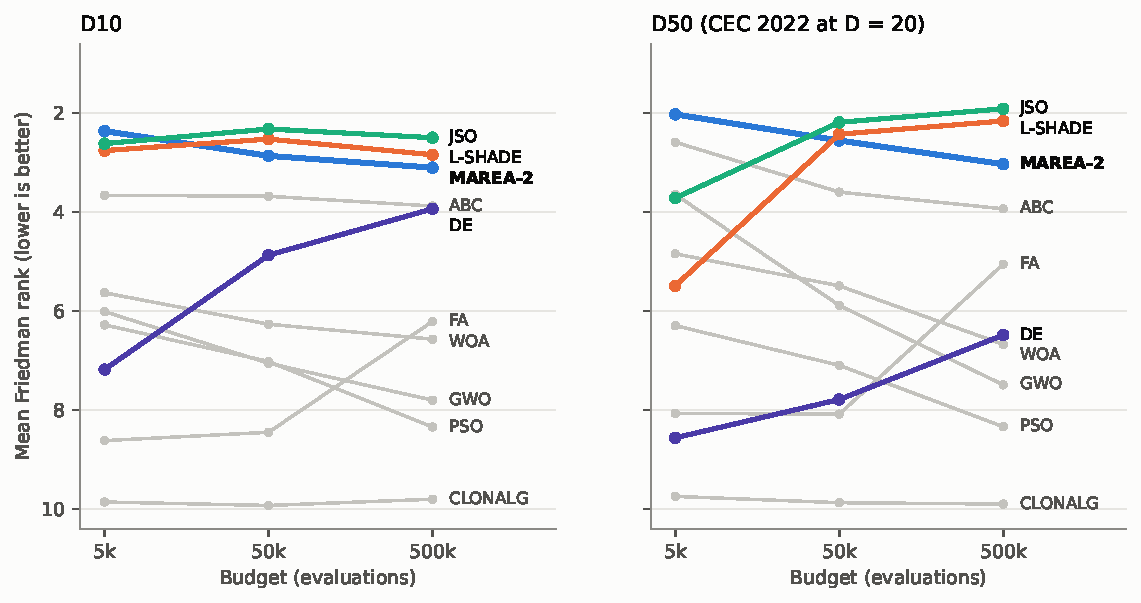
\includegraphics[width=\linewidth]{figs/fig_rangos.pdf}
  \caption{Mean Friedman rank of each algorithm as a function of the budget.}
  \label{fig:ranks}
\end{figure}

The ranks of jSO and L-SHADE improve with the budget, most visibly in D50,
where L-SHADE moves from sixth place at 5,000 evaluations to second at 500,000.
MAREA-2 follows the opposite trend. This pattern suggests that its strength lies
in reaching good regions quickly, while the two DE variants make better use of
long runs. The ranking does not depend on the choice of the mean as the score:
with the median of the 51 runs, MAREA-2 keeps the same position in all six
combinations. The positions are also stable across suites. MAREA-2 is never below third place in any of the 18 rankings by suite and
combination. It ranks first on CEC~2014 in D10 at 5,000 evaluations, on
CEC~2017 in D50 at the same budget, and on CEC~2022 in D10 at 50,000
evaluations. Across these 18
rankings, its mean position is 2.28 with a standard deviation of 0.75, while
jSO obtains 1.61 and 1.04, and L-SHADE obtains 2.72 and 1.36.

Figure~\ref{fig:cd} shows the critical difference diagrams of the Nemenyi test.
Each diagram places the algorithms on the axis of mean ranks, and a thick
horizontal bar joins algorithms whose ranks differ by less than the critical
difference of 1.61. In D50 at 5,000 evaluations, MAREA-2 is significantly
better than every algorithm except ABC. In the other five combinations, the
test does not separate MAREA-2 from jSO, L-SHADE, and ABC, and in D10 at
500,000 evaluations not from DE either. Shaffer's procedure agrees on every
comparison that involves MAREA-2. Its differences against L-SHADE
($p = 2.6\times10^{-10}$) and jSO ($p = 0.012$) are significant only in D50 at
5,000 evaluations, and its difference against ABC is never significant. Rank
tests over 71 functions and ten algorithms have limited power for algorithms
with close ranks, so we complement them with pairwise tests in
Section~\ref{sec:pairwise}.

\begin{figure}[t]
  \centering
  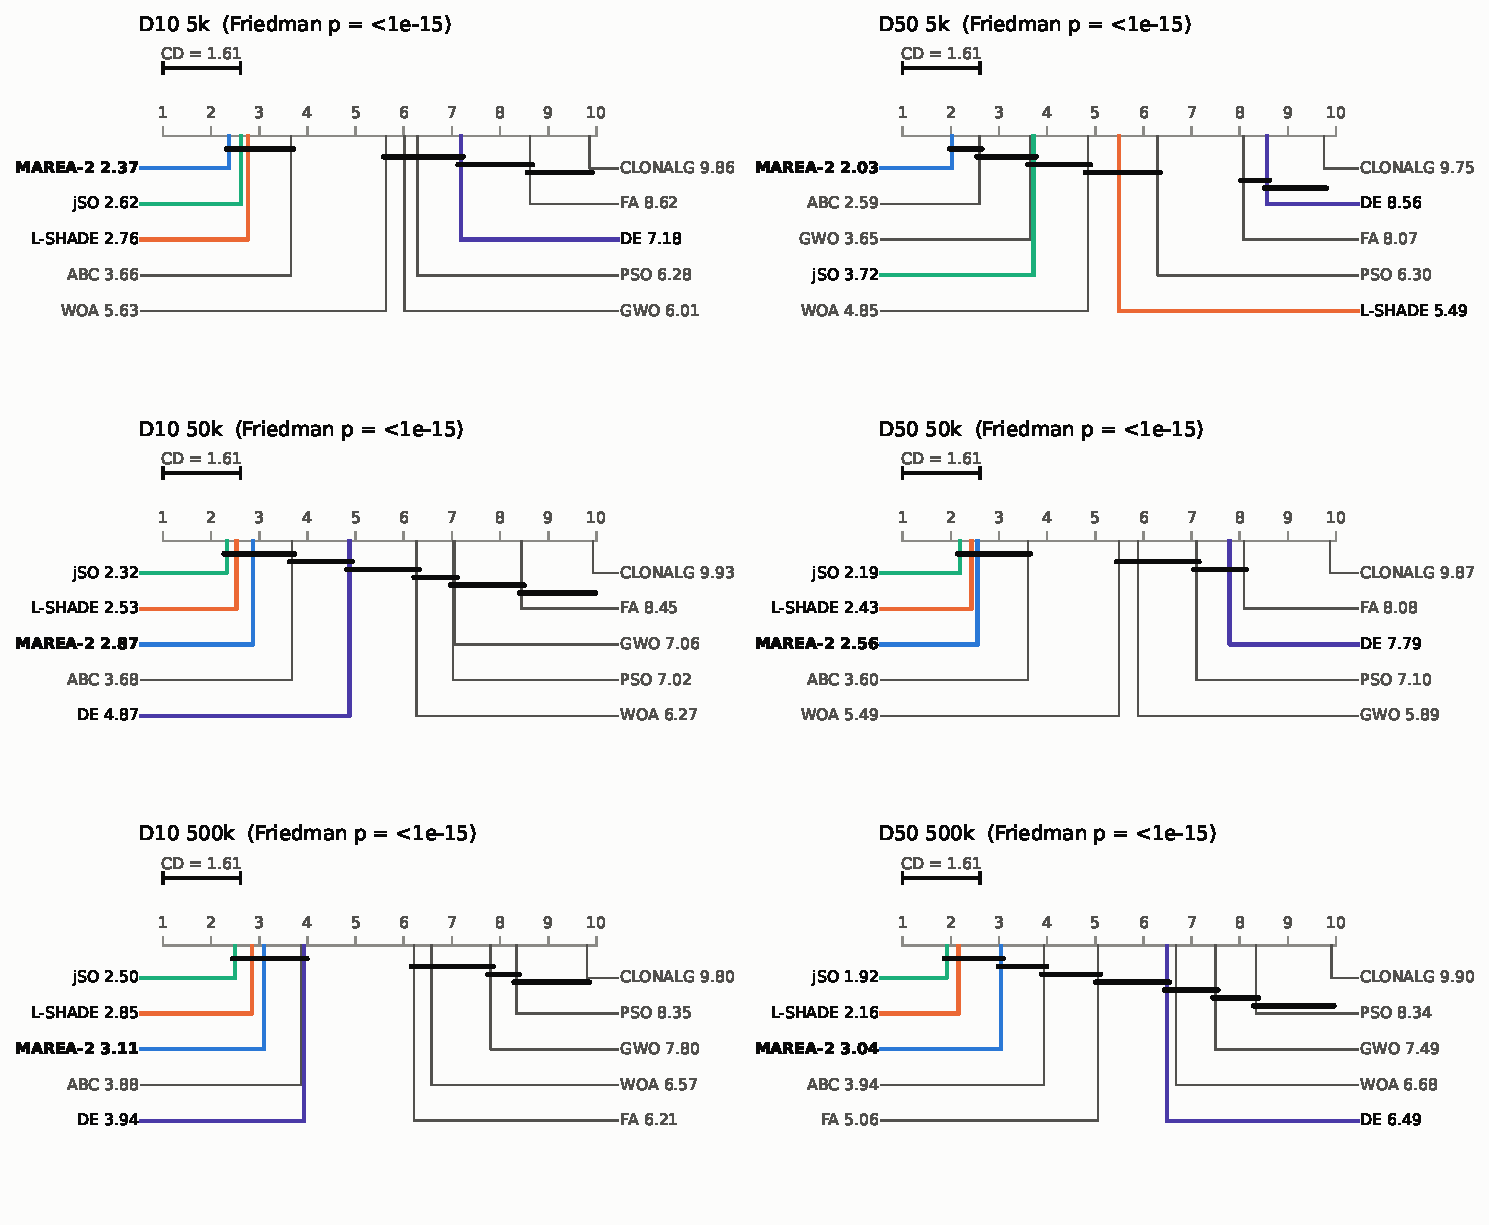
\includegraphics[width=\linewidth]{figs/fig_cd_nemenyi.pdf}
  \caption{Critical difference diagrams of the Nemenyi test for the six combinations of dimension setting and budget.}
  \label{fig:cd}
\end{figure}

\subsection{Pairwise comparisons}
\label{sec:pairwise}

Figure~\ref{fig:wtl} and Table~\ref{tab:wtl} count, per function, the
significant differences between MAREA-2 and each competitor. In the figure,
each bar splits the 71 functions into wins, ties, and losses of MAREA-2.
Table~\ref{tab:signedrank} gives the signed-rank test over the 71 mean errors.
Against the seven classical metaheuristics, MAREA-2 is significantly better in
40 of the 42 signed-rank comparisons. The first exception is ABC in D50 at 5,000 evaluations ($p = 0.676$), where ABC
wins on 34 functions and MAREA-2 on 26. The second is DE in D10 at 500,000
evaluations ($p = 0.064$), where MAREA-2 wins on 32 functions and DE on 23.

\begin{figure}[t]
  \centering
  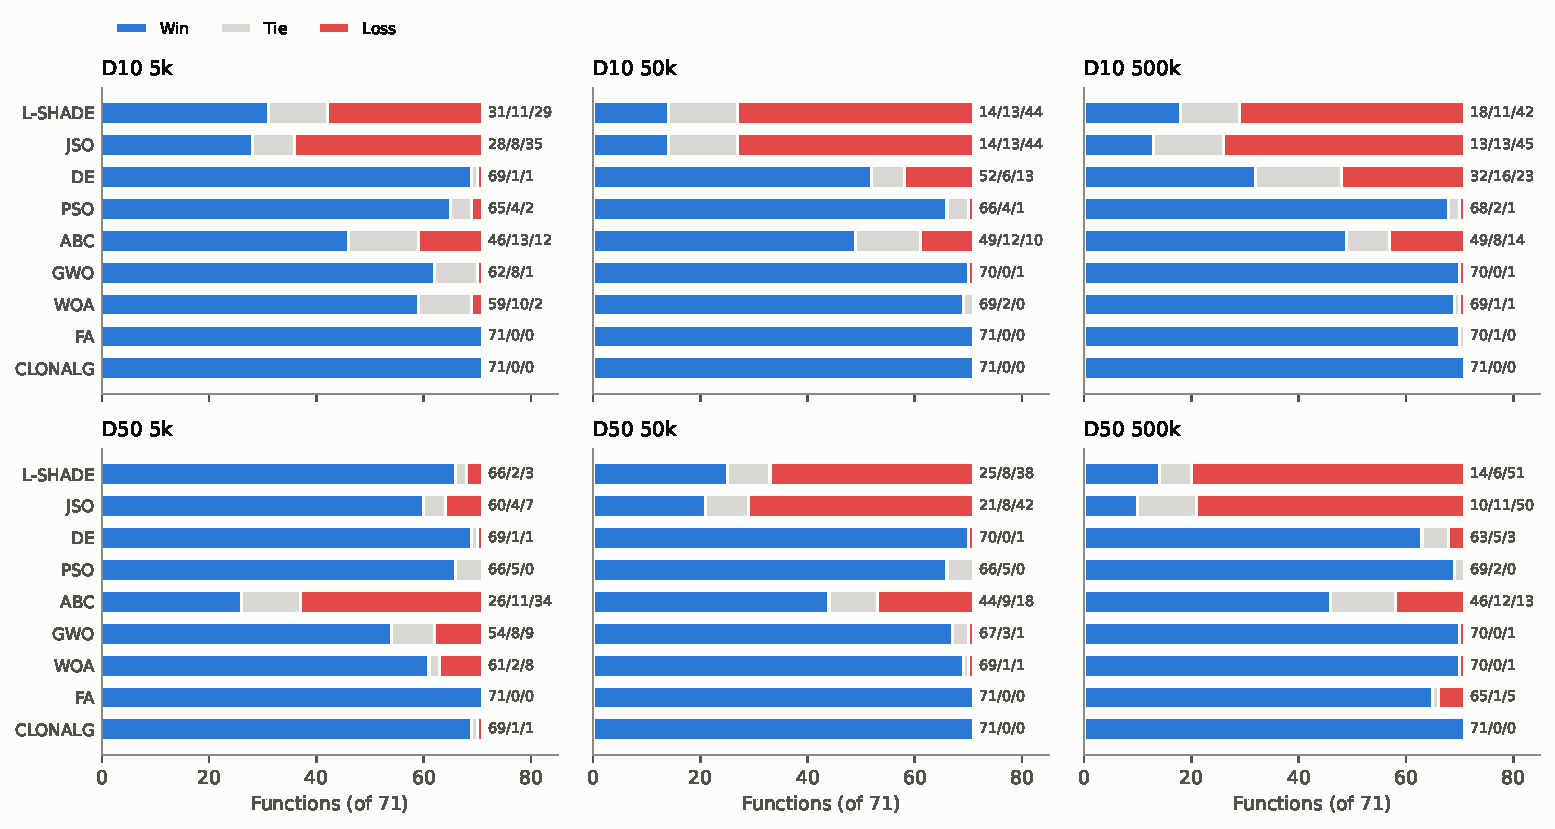
\includegraphics[width=\linewidth]{figs/fig_wtl.pdf}
  \caption{Wins, ties, and losses of MAREA-2 against each competitor.}
  \label{fig:wtl}
\end{figure}

% Generated by generar_tablas_en.py from paper/tablas; do not edit by hand.
\begin{table}[t]
\centering
\small
\caption{Wins, ties, and losses of MAREA-2 against each competitor over the 71 functions.}
\label{tab:wtl}
\begin{tabular}{lcccccc}
\toprule
Competitor & D10 5k & D10 50k & D10 500k & D50 5k & D50 50k & D50 500k \\
\midrule
L-SHADE & 31/11/29 & 14/13/44 & 18/11/42 & 66/2/3 & 25/8/38 & 14/6/51 \\
jSO & 28/8/35 & 14/13/44 & 13/13/45 & 60/4/7 & 21/8/42 & 10/11/50 \\
DE & 69/1/1 & 52/6/13 & 32/16/23 & 69/1/1 & 70/0/1 & 63/5/3 \\
PSO & 65/4/2 & 66/4/1 & 68/2/1 & 66/5/0 & 66/5/0 & 69/2/0 \\
ABC & 46/13/12 & 49/12/10 & 49/8/14 & 26/11/34 & 44/9/18 & 46/12/13 \\
GWO & 62/8/1 & 70/0/1 & 70/0/1 & 54/8/9 & 67/3/1 & 70/0/1 \\
WOA & 59/10/2 & 69/2/0 & 69/1/1 & 61/2/8 & 69/1/1 & 70/0/1 \\
FA & 71/0/0 & 71/0/0 & 70/1/0 & 71/0/0 & 71/0/0 & 65/1/5 \\
CLONALG & 71/0/0 & 71/0/0 & 71/0/0 & 69/1/1 & 71/0/0 & 71/0/0 \\
\bottomrule
\end{tabular}
\par\smallskip\footnotesize Per function, Wilcoxon rank-sum test on 51 runs with $\alpha = 0.05$; the sign of a significant difference is given by the means.
\end{table}

% Generated by generar_tablas_en.py from paper/tablas; do not edit by hand.
\begin{table}[t]
\centering
\footnotesize
\caption{Holm-adjusted $p$-values of the Wilcoxon signed-rank test between MAREA-2 and each competitor.}
\label{tab:signedrank}
\begin{tabular}{lcccccc}
\toprule
Competitor & D10 5k & D10 50k & D10 500k & D50 5k & D50 50k & D50 500k \\
\midrule
L-SHADE & 0.281 & 0.032$^{-}$ & 0.120 & $1.61\times10^{-11}$$^{+}$ & 0.015$^{-}$ & $1.93\times10^{-6}$$^{-}$ \\
jSO & 0.036$^{-}$ & 0.032$^{-}$ & 0.120 & $1.22\times10^{-9}$$^{+}$ & 0.001$^{-}$ & $4.32\times10^{-7}$$^{-}$ \\
DE & $3.13\times10^{-12}$$^{+}$ & 0.016$^{+}$ & 0.064 & $2.51\times10^{-12}$$^{+}$ & $2.19\times10^{-12}$$^{+}$ & $7.26\times10^{-11}$$^{+}$ \\
PSO & $4.31\times10^{-12}$$^{+}$ & $2.19\times10^{-12}$$^{+}$ & $2.19\times10^{-12}$$^{+}$ & $3.86\times10^{-12}$$^{+}$ & $2.19\times10^{-12}$$^{+}$ & $2.19\times10^{-12}$$^{+}$ \\
ABC & $4.92\times10^{-5}$$^{+}$ & $1.74\times10^{-4}$$^{+}$ & $9.38\times10^{-4}$$^{+}$ & 0.676 & 0.001$^{+}$ & 0.005$^{+}$ \\
GWO & $2.72\times10^{-12}$$^{+}$ & $3.80\times10^{-12}$$^{+}$ & $3.55\times10^{-12}$$^{+}$ & $4.06\times10^{-8}$$^{+}$ & $2.37\times10^{-12}$$^{+}$ & $3.40\times10^{-12}$$^{+}$ \\
WOA & $2.10\times10^{-11}$$^{+}$ & $3.70\times10^{-12}$$^{+}$ & $3.55\times10^{-12}$$^{+}$ & $6.21\times10^{-10}$$^{+}$ & $2.19\times10^{-12}$$^{+}$ & $2.20\times10^{-12}$$^{+}$ \\
FA & $2.19\times10^{-12}$$^{+}$ & $2.19\times10^{-12}$$^{+}$ & $2.19\times10^{-12}$$^{+}$ & $2.19\times10^{-12}$$^{+}$ & $2.19\times10^{-12}$$^{+}$ & $7.26\times10^{-11}$$^{+}$ \\
CLONALG & $2.19\times10^{-12}$$^{+}$ & $2.19\times10^{-12}$$^{+}$ & $2.19\times10^{-12}$$^{+}$ & $2.51\times10^{-12}$$^{+}$ & $2.19\times10^{-12}$$^{+}$ & $2.19\times10^{-12}$$^{+}$ \\
\bottomrule
\end{tabular}
\par\smallskip\footnotesize The test pairs the 71 mean errors. $^{+}$ and $^{-}$ mark a significant difference ($\alpha = 0.05$) in favor of or against MAREA-2.
\end{table}


Against jSO and L-SHADE, the outcome depends on the budget. In D50 at 5,000
evaluations, MAREA-2 wins on 66 functions against L-SHADE and on 60 against
jSO, with $p < 10^{-8}$ in both signed-rank tests. In D10 at the same budget,
the counts are balanced, 31/11/29 against L-SHADE and 28/8/35 against jSO, and
only the difference against jSO is significant ($p = 0.036$). At 50,000 and
500,000 evaluations, jSO and L-SHADE win on 38 to 51 functions and MAREA-2 on
10 to 25. The signed-rank test favors the two DE variants in six of these eight
comparisons, and D10 at 500,000 evaluations is the exception, with $p = 0.120$
against both.

Table~\ref{tab:class} breaks the comparison with L-SHADE and jSO down by
function class. At 5,000 evaluations, MAREA-2 wins on most multimodal
functions in both settings, for example on 18 of 24 against jSO in D10 and on
21 of 24 in D50. In D50, it also wins on most hybrid and composition functions.
At the larger budgets, the gap concentrates on the hybrid functions, where jSO
wins on 15 to 18 of the 19 functions, and on the unimodal functions. The
composition functions remain closer. In D10, MAREA-2 wins on 11 and 12 of the 22 composition functions against
L-SHADE at 50,000 and 500,000 evaluations. Its record against jSO at 500,000
evaluations is 8/5/9.

% Generated by generar_tablas_en.py from paper/tablas; do not edit by hand.
\begin{table}[t]
\centering
\footnotesize
\caption{Wins, ties, and losses of MAREA-2 against L-SHADE and jSO by function class.}
\label{tab:class}
\begin{tabular}{llcccccc}
\toprule
Competitor & Class ($n$) & D10 5k & D10 50k & D10 500k & D50 5k & D50 50k & D50 500k \\
\midrule
L-SHADE & Unimodal (6) & 3/1/2 & 0/2/4 & 0/2/4 & 6/0/0 & 0/2/4 & 0/2/4 \\
L-SHADE & Multimodal (24) & 14/7/3 & 3/5/16 & 5/6/13 & 23/1/0 & 15/2/7 & 6/3/15 \\
L-SHADE & Hybrid (19) & 4/2/13 & 0/4/15 & 1/1/17 & 19/0/0 & 2/3/14 & 0/1/18 \\
L-SHADE & Composition (22) & 10/1/11 & 11/2/9 & 12/2/8 & 18/1/3 & 8/1/13 & 8/0/14 \\
jSO & Unimodal (6) & 0/0/6 & 0/2/4 & 0/2/4 & 4/0/2 & 0/1/5 & 0/2/4 \\
jSO & Multimodal (24) & 18/3/3 & 6/4/14 & 3/6/15 & 21/2/1 & 14/3/7 & 3/7/14 \\
jSO & Hybrid (19) & 4/0/15 & 2/2/15 & 2/0/17 & 17/1/1 & 1/2/16 & 1/0/18 \\
jSO & Composition (22) & 6/5/11 & 6/5/11 & 8/5/9 & 18/1/3 & 6/2/14 & 6/2/14 \\
\bottomrule
\end{tabular}
\par\smallskip\footnotesize Same test as Table~\ref{tab:wtl}. The class follows the definitions of each suite.
\end{table}


These patterns agree with the design of MAREA-2. The logistic schedule removes
half of the planned reduction within the first 31\,\% of the budget, so the
evaluations concentrate early on fewer and better individuals. The
success-based step factor enlarges the steps while improvements are frequent.
Both features favor a fast descent, which pays off at small budgets. A
plausible reason for the gap on hybrid functions at large budgets is that
these functions combine different base functions over groups of variables.
L-SHADE and jSO adapt their mutation and crossover parameters per individual
from a historical memory, whereas MAREA-2 adapts a single crossover rate and
learns no covariance. This identifies per-individual parameter adaptation as
the next extension to test.

\placeholder{Figure~\ref{fig:convergence}, pending new runs (convergence
curves). Content: median best error against the number of evaluations, on a
log scale, for the ten algorithms, on one or two functions per class in D10 and
D50 at 500,000 evaluations, with the seeds of the protocol. Purpose: show where
MAREA-2 gains early and where L-SHADE and jSO overtake it. Suggested caption:
``Median convergence of the ten algorithms on representative functions.''}
\begin{figure}[h]
  \caption{\pend{Median convergence of the ten algorithms on representative functions.}}
  \label{fig:convergence}
\end{figure}

\pend{Paragraph on Figure~\ref{fig:convergence} to be written when the
convergence runs exist. It will state at how many evaluations jSO and L-SHADE
overtake MAREA-2 on each class, which is \XX\ in D10 and \XX\ in D50.}

\subsection{Ablation}
\label{sec:ablation}

Table~\ref{tab:ablation} summarizes the ablation that fixed the configuration
of MAREA-2. The study used 15 independent runs per configuration on the 71
functions, mostly at 5,000 and 50,000 evaluations, and compared configurations
with the per-function rank-sum test. The design started from a version with
spatial microcolonies, in which clusters of individuals had their own best
point and mean. Removing them improved the results in D50 at every budget
tested, with 48, 51, and 38 functions in favor of the version without them, so
we dropped them. All later comparisons use the version without microcolonies.
The final configuration adds the adaptive crossover of
Equation~\eqref{eq:crossover}. It won on 29 and 24 functions in D10 at 50,000 and 500,000 evaluations,
against 7 and 11 losses. In D50, the counts were mixed.

% Generated by generar_tablas_en.py from paper/tablas; do not edit by hand.
\begin{table*}[t]
\centering
\scriptsize
\caption{Ablation of the components of MAREA-2.}
\label{tab:ablation}
\begin{tabular}{>{\raggedright\arraybackslash}p{0.2\linewidth}lcccccc>{\raggedright\arraybackslash}p{0.2\linewidth}}
\toprule
Component & Base & D10 5k & D10 50k & D10 500k & D50 5k & D50 50k & D50 500k & Decision \\
\midrule
Microcolonies & Initial & 0/48/23 & 5/48/18 & 8/56/7 & 1/22/48 & 2/18/51 & 1/32/38 & Removed: worse in D50, and in D10 at 5k and 50k \\
Stagnation-triggered dispersal & Initial & 0/71/0 & 11/53/7 & n/r & 0/71/0 & 6/65/0 & n/r & Kept; nearly inert \\
Success-based step factor (R2) & Initial & 21/48/2 & 7/62/2 & n/r & 43/28/0 & 41/27/3 & n/r & Kept: helps, mainly in D50 \\
Success-based step factor (R2) & No col. & n/r & 11/59/1 & 8/61/2 & n/r & 47/24/0 & 28/33/10 & Confirmed at 500k without microcolonies \\
Logistic vs.\ constant population (R1) & Initial & 34/35/2 & 10/61/0 & n/r & 53/18/0 & 41/29/1 & n/r & Kept: helps at 5k and in D50 \\
Logistic vs.\ linear schedule (R1) & Initial & 4/67/0 & 4/65/2 & n/r & 10/61/0 & 11/60/0 & n/r & Logistic $\geq$ linear; kept \\
Logistic vs.\ Gompertz schedule (R1) & Initial & 0/69/2 & 1/64/6 & n/r & 0/59/12 & 0/62/9 & n/r & With microcolonies, Gompertz slightly better in D50 \\
Logistic vs.\ Gompertz schedule (R1) & No col. & 3/68/0 & 4/63/4 & n/r & 3/67/1 & 10/58/3 & n/r & Without microcolonies, logistic $\geq$ Gompertz; kept \\
Step scaled by population spread & Initial & 2/42/27 & 25/37/9 & n/r & 7/44/20 & 21/23/27 & n/r & Mixed, trails at 5k; kept \\
Greedy selection & Initial & 61/7/3 & 65/5/1 & n/r & 60/5/6 & 66/3/2 & n/r & Kept: essential \\
Archive of exhausted regions & Initial & 0/71/0 & 1/70/0 & n/r & 0/71/0 & 0/71/0 & n/r & Inert; retained \\
Lag phase & Initial & 1/69/1 & 0/70/1 & n/r & 1/68/2 & 3/67/1 & n/r & Inert; retained \\
Archive and lag phase together & No col. & 0/67/4 & 2/68/1 & n/r & 2/66/3 & 4/65/2 & n/r & Inert; retained \\
Dispersal limit shortened at 5k & No col. & 0/70/1 & n/r & n/r & 0/68/3 & n/r & n/r & Inert; not adopted \\
Student-$t$ vs.\ Gaussian term (R3) & Initial & 2/66/3 & 8/61/2 & n/r & 0/68/3 & 2/63/6 & n/r & Neutral; Gaussian slightly better in D50 \\
Student-$t$ vs.\ Gaussian, coordinate-wise only (R3) & No col.\textsuperscript{a} & 7/58/6 & 15/51/5 & n/r & 10/56/5 & 9/53/9 & n/r & Student-$t$ $\geq$ Gaussian; kept \\
Difference vector vs.\ coordinate-wise only & Initial & 15/31/25 & 22/44/5 & 26/42/3 & 4/11/56 & 7/15/49 & 17/27/27 & Coordinate-wise better in D50 at 5k and 50k; difference vector kept \\
Difference vector vs.\ coordinate-wise only & No col. & 18/34/19 & 34/34/3 & 30/39/2 & 6/17/48 & 15/16/40 & 25/31/15 & Difference vector better at 500k in both settings \\
No second-stage changes vs.\ all of them & No col. & 23/27/21 & 35/34/2 & n/r & 5/15/51 & 16/14/41 & n/r & Not adopted; the criterion was the 500k result in both settings \\
Adaptive partial transfer (crossover) & Final & n/r & 29/35/7 & 24/36/11 & n/r & 34/15/22 & 23/25/23 & Adopted: better in D10, mixed in D50 \\
Adaptive vs.\ fixed rate 0.5 & Final & n/r & 19/42/10 & n/r & n/r & 20/23/28 & n/r & Adaptive better in D10; fixed slightly better in D50 \\
Full design vs.\ ancestor without the laws & Initial & 53/14/4 & 65/4/2 & n/r & 42/17/12 & 34/11/26 & n/r & Full design better in all four cells \\
\bottomrule
\end{tabular}
\par\smallskip\footnotesize A row named after a component compares the configuration with it against the one without it, and a row of the form A vs.\ B compares A against B. Each cell gives wins, ties, and losses of the first configuration (Wilcoxon rank-sum on 15 runs per arm, $\alpha = 0.05$). Base: Initial is the design with microcolonies, No col.\ removes them, and Final is MAREA-2. \textsuperscript{a}Without microcolonies and with the coordinate-wise term only. n/r: not run.
\end{table*}


The logistic schedule, which implements R1, improved on a constant population
on 34 and 53 functions at 5,000 evaluations in D10 and D50. It also improved
on 41 functions in D50 at 50,000 evaluations, with at most two losses in each
case.
Against the linear reduction of L-SHADE, it won on 4 to 11 functions and lost
on at most two, so the fitted shape is at least as good as the linear one.
Against a Gompertz schedule, the result depends on the rest of the design. With
microcolonies, the Gompertz schedule was slightly better in D50, with 12 and 9
functions in its favor, and without them the logistic won on 3 to 10 functions
and lost on at most 4.

The success-based step factor, which implements the first part of R2, helped
most in D50, where it won on 43 and 41 functions at 5,000 and 50,000
evaluations with at most three losses. Repeated without microcolonies, the
comparison confirmed it at 500,000 evaluations, with 28 wins and 10 losses in
D50 and 8 wins and 2 losses in D10. The stagnation-triggered dispersal, the
second part of R2, was nearly inert and changed at most 18 functions in any
combination.

The Student-$t$ shape, which implements R3, had a small effect. As the
coordinate-wise term of the initial design, it was neutral against a Gaussian
term, with at most 8 wins and 6 losses. When the coordinate-wise term was the
only perturbation, the Student-$t$ version won on 7 to 15 functions and lost on
5 to 9, which favors the heavy tail without a large margin.

Among the components that do not come from the biological model, greedy
selection had the largest effect, with 60 to 66 wins in the four combinations.
The archive of exhausted regions and the lag phase were inert and changed at
most 6 functions, alone or together; we kept them because removing them did
not change the results. Finally, the complete initial design improved on its
ancestor, in which every component is switched off, on 34 to 65 functions,
although in D50 at 50,000 evaluations it also trailed on 26.

\subsection{Limitations}
\label{sec:limitations}

Five aspects limit the scope of these results. First, the ablation and the
evaluation used the same 71 functions, so the configuration of MAREA-2 was
chosen on the benchmark on which it is evaluated, whereas the competitors used
their published parameters. Second, MAREA-2 retains three components that the
ablation found inert or nearly inert, namely the archive, the lag phase, and
the dispersal, and a more parsimonious version would drop them. Third, the
second law enters MAREA-2 only as a direction, and the target success rate
comes from evolution strategies and not from the biological data. Fourth, our
implementation of jSO differs from its published results on several
composition functions of CEC~2017, as described in Section~\ref{sec:setup}, so
comparisons on that class carry the uncertainty of the benchmark
implementation. Fifth, the study covers bound-constrained synthetic functions
only, and constrained or real-world problems remain to be tested.
\pend{Solving times, a random search baseline, and a sensitivity analysis on a
suite different from the evaluation suites are planned and will be reported
here with their numbers (\XX).}

% =============================================================================
\section{Conclusions}
\label{sec:conclusions}

We proposed MAREA-2, a population-based metaheuristic whose rules come from
three laws measured in the marine bacterium \emph{Cobetia} sp.\ MM1IDA2H-1. The fitted logistic growth curve became a population size schedule, and the
heavy-tailed variability of the growth data became the shape of the
perturbation. The trade-off between planktonic growth and biofilm formation
became a success-based step factor and a stagnation-triggered dispersal. We described every
rule in standard optimization terms, named the mechanism it is equivalent to,
and tested it in an ablation study, which also removed a microcolony structure
from an earlier design.

On 71 functions from three CEC suites, MAREA-2 obtained the best mean rank at
5,000 evaluations in both dimension settings. At 50,000 and 500,000
evaluations, it ranked third, after jSO and L-SHADE, which led on hybrid and
unimodal functions, while the comparison on composition functions remained
close. Against seven classical metaheuristics, MAREA-2 was significantly better
in 40 of 42 signed-rank comparisons. The ablation attributes the clearest
gains to the logistic schedule and the success-based step factor, and a
smaller one to the heavy-tailed perturbation. These results position MAREA-2 as
an optimizer for small and medium budgets, and they show that measured laws of
an organism can be turned into rules that an ablation can test.

Three lines of future work follow from the results. The first is
per-individual adaptation of the step and crossover parameters, which the
comparison by function class identifies as the setting where MAREA-2 has most
room to grow. The second is a configuration study on a suite separate from the
evaluation suites, together with convergence curves, solving times, and
constrained problems. The third is the use of the covariate effects of the
growth model, such as the dependence of the growth scale on temperature, as
additional adaptive rules.

\section*{Data and code availability}

The code of all algorithms, the error of every run, and the analysis scripts
will be deposited in a public repository with a DOI
\pend{(repository and DOI to be added at submission)}.

\bibliographystyle{elsarticle-num}
\bibliography{refs}

\end{document}
